\documentclass[11pt,a4paper]{article}

% =============================================================================
% PACKAGES
% =============================================================================
\usepackage[utf8]{inputenc}
\usepackage[T1]{fontenc}
\usepackage{geometry}
\usepackage{amsmath,amssymb}
\usepackage{booktabs}
\usepackage{hyperref}
\usepackage{enumitem}
\usepackage{tikz}
\usetikzlibrary{shapes,arrows.meta,positioning,calc,fit}

\geometry{margin=1in}

% =============================================================================
% CUSTOM COMMANDS
% =============================================================================
\newcommand{\R}{\mathbb{R}}
\newcommand{\bz}{\mathbf{z}}
\newcommand{\bx}{\mathbf{x}}
\newcommand{\bW}{\mathbf{W}}
\newcommand{\bb}{\mathbf{b}}
\newcommand{\bh}{\mathbf{h}}

\title{Latent MLP --- Stage~2 Architecture\\[0.5em]
\large Mapping Physical Parameters to Latent Codes}
\author{Project 2: Nonlinear Data-Driven Reduced Order Models}
\date{}

\begin{document}
\maketitle

% ============================================================================
\section{Purpose and Context}
% ============================================================================

The Latent MLP is the second stage in a two-stage parametric reduced-order
model (ROM) pipeline:
%
\begin{enumerate}[leftmargin=2em]
  \item \textbf{Stage~1 --- Convolutional Autoencoder (CAE):}  
    A trained CAE compresses high-dimensional spatial fields
    $\mathbf{u} \in \R^{C \times H \times W}$ into compact latent codes
    $\bz \in \R^{d}$.  The CAE is trained on snapshot data and then
    \emph{frozen}.
  \item \textbf{Stage~2 --- Latent MLP (this network):}  
    A small Multi-Layer Perceptron (MLP) learns to predict the latent codes
    $\bz$ directly from physical parameters $(\mu, t)$, bypassing the
    expensive encoder at inference time.
\end{enumerate}

At \textbf{inference} the pipeline is:
\[
  (\mu,\, t)
  \;\xrightarrow{\text{MLP}}\;
  \hat{\bz}
  \;\xrightarrow{\text{Decoder}}\;
  \hat{\mathbf{u}}(\mathbf{x})
\]
where $\mu$ is the physical parameter (e.g.\ wave speed) and $t$ is the
time instant.

% ============================================================================
\section{Input: Physical Parameters \texorpdfstring{$(\mu, t)$}{(mu, t)}}
% ============================================================================

Each snapshot in the database is uniquely identified by a simulation
case (parametrized by $\mu$) and a time step $t$.  The MLP receives
these as a single input vector:
\[
  \bx = \begin{pmatrix} \mu \\ t \end{pmatrix} \in \R^{2}
\]
More generally, if the PDE has $p$ parameters $(\mu_1,\ldots,\mu_p)$,
the input dimension is $p+1$ (parameters plus time):
\[
  \bx = (\mu_1,\;\mu_2,\;\ldots,\;\mu_p,\;t)^{\!\top} \in \R^{p+1}.
\]

\paragraph{Input normalization (z-score).}
Before entering the network, each input column is standardized using
training-set statistics:
\[
  \hat{x}_j = \frac{x_j - \bar{x}_j}{\sigma_{x_j}}
  ,\qquad j = 1,\ldots, p+1
\]
where $\bar{x}_j$ and $\sigma_{x_j}$ are the mean and standard
deviation of column $j$ computed over the training set only.
This ensures that every input feature has approximately zero mean
and unit variance, which helps gradient-based optimization converge
faster and more stably.

% ============================================================================
\section{Network Architecture}
% ============================================================================

The MLP has a simple feedforward architecture with two hidden layers:

\[
  \bx \in \R^{n_{\mathrm{in}}}
  \;\xrightarrow{\bW^{(1)},\;\bb^{(1)}}\;
  \bh^{(1)} \in \R^{H}
  \;\xrightarrow{\;\sigma\;}\;
  \bh^{(1)}_{\text{act}}
  \;\xrightarrow{\bW^{(2)},\;\bb^{(2)}}\;
  \bh^{(2)} \in \R^{H}
  \;\xrightarrow{\;\sigma\;}\;
  \bh^{(2)}_{\text{act}}
  \;\xrightarrow{\bW^{(3)},\;\bb^{(3)}}\;
  \hat{\bz} \in \R^{d}
\]

where $n_{\mathrm{in}} = p + 1$ is the input dimension, $H$ is the hidden
dimension, $d$ is the latent dimension, and $\sigma$ denotes the ReLU
activation function.

% ----------------------------------------------------------------------------
\subsection{Layer-by-Layer Breakdown}
% ----------------------------------------------------------------------------

\paragraph{Layer~1 --- Linear transformation.}
The normalized input $\hat{\bx} \in \R^{n_{\mathrm{in}}}$ is multiplied
by a weight matrix and shifted by a bias vector:
\[
  \bh^{(1)} = \bW^{(1)} \hat{\bx} + \bb^{(1)}
  ,\qquad
  \bW^{(1)} \in \R^{H \times n_{\mathrm{in}}},\;
  \bb^{(1)} \in \R^{H}.
\]
This is a standard \emph{affine transformation}: every output neuron
computes a weighted sum of all inputs plus a bias.  With
$n_{\mathrm{in}}=2$ and $H=64$ this layer has $2\times64 + 64 = 192$
learnable parameters.

\paragraph{Activation~1 --- ReLU.}
The Rectified Linear Unit applies an element-wise nonlinearity:
\[
  \bh^{(1)}_{\text{act}} = \mathrm{ReLU}\!\bigl(\bh^{(1)}\bigr)
  = \max\!\bigl(0,\;\bh^{(1)}\bigr).
\]
For each component $h_i$: if $h_i > 0$ it passes through unchanged;
if $h_i \le 0$ it is set to zero.  Key properties:
\begin{itemize}[leftmargin=2em]
  \item Introduces \textbf{nonlinearity} --- without it, stacking
    linear layers would collapse to a single linear map, and the
    network could not approximate nonlinear functions.
  \item Computationally cheap (just a threshold).
  \item Gradients are either 0 or 1, avoiding the vanishing gradient
    problem of sigmoid/tanh for deep networks.
  \item \textbf{No learnable parameters} --- it is a fixed pointwise
    operation.
\end{itemize}

\paragraph{Layer~2 --- Linear transformation.}
\[
  \bh^{(2)} = \bW^{(2)} \bh^{(1)}_{\text{act}} + \bb^{(2)}
  ,\qquad
  \bW^{(2)} \in \R^{H \times H},\;
  \bb^{(2)} \in \R^{H}.
\]
With $H=64$: $64\times64 + 64 = 4{,}160$ parameters.

\paragraph{Activation~2 --- ReLU.}
\[
  \bh^{(2)}_{\text{act}} = \mathrm{ReLU}\!\bigl(\bh^{(2)}\bigr).
\]
Same pointwise operation as before, applied to the second hidden layer.

\paragraph{Layer~3 --- Output linear transformation.}
\[
  \hat{\bz} = \bW^{(3)} \bh^{(2)}_{\text{act}} + \bb^{(3)}
  ,\qquad
  \bW^{(3)} \in \R^{d \times H},\;
  \bb^{(3)} \in \R^{d}.
\]
With $H=64$ and $d=4$: $64\times4 + 4 = 260$ parameters.

\textbf{No output activation} is applied.  The latent codes $\bz$
produced by the encoder can take any real value, so the MLP output
must be unconstrained.

% ----------------------------------------------------------------------------
\subsection{Summary Table}
% ----------------------------------------------------------------------------

\begin{table}[h]
\centering
\caption{MLP architecture summary (default: $n_{\mathrm{in}}=2$, $H=64$, $d=4$).}
\label{tab:mlp-arch}
\begin{tabular}{@{}llccc@{}}
\toprule
\textbf{Layer} & \textbf{Operation} & \textbf{Input dim} & \textbf{Output dim} & \textbf{Parameters} \\
\midrule
1 & $\bW^{(1)}\bx + \bb^{(1)}$ & $n_{\mathrm{in}}$ & $H$ & $n_{\mathrm{in}} \cdot H + H$ \\
  & ReLU & $H$ & $H$ & 0 \\
2 & $\bW^{(2)}\bh + \bb^{(2)}$ & $H$ & $H$ & $H^2 + H$ \\
  & ReLU & $H$ & $H$ & 0 \\
3 & $\bW^{(3)}\bh + \bb^{(3)}$ & $H$ & $d$ & $H \cdot d + d$ \\
\midrule
\multicolumn{4}{@{}l}{\textbf{Total (CNN encoder, $d=4$)}} & 4{,}612 \\
\multicolumn{4}{@{}l}{\textbf{Total (KTH encoder, $d=1024$)}} & 70{,}848 \\
\bottomrule
\end{tabular}
\end{table}

The total parameter count is:
\[
  N_{\text{params}} = n_{\mathrm{in}} \cdot H + H + H^2 + H + H \cdot d + d
  = (n_{\mathrm{in}} + H + d)\,H + (H + d).
\]

% ----------------------------------------------------------------------------
\subsection{Who Decides These Numbers?  Hyperparameters vs.\ Architecture}
\label{sec:hyperparams}
% ----------------------------------------------------------------------------

A common source of confusion: \emph{``Where does 64 come from? And is
the network 3 layers or 2?''}

\paragraph{Hidden dimension $H = 64$.}
This is a \textbf{hyperparameter} --- a design choice made by the user
\emph{before} training, not something the network learns.  It is set in
\texttt{train\_latent\_mlp.py}:
\begin{center}
\texttt{HIDDEN\_DIM = 64}
\end{center}
There is no formula that dictates $H=64$.  The value is chosen by the
practitioner based on experience, problem complexity, and
experimentation. Common considerations:
\begin{itemize}[leftmargin=2em]
  \item \textbf{Too small} ($H=4$): The network cannot capture the
    nonlinear mapping and underfits.
  \item \textbf{Too large} ($H=1024$): The network has far more
    capacity than needed for a $\R^2 \to \R^d$ mapping, wastes memory,
    and may overfit.
  \item \textbf{$H=64$} is a reasonable middle ground for a smooth,
    low-dimensional regression problem.  It could equally have been 32
    or 128 --- the choice is empirical.
\end{itemize}

\paragraph{How many layers?  The ``3 layers'' question.}
The terminology can be confusing because there are two common counting
conventions:

\begin{table}[h]
\centering
\begin{tabular}{@{}lcc@{}}
\toprule
\textbf{Counting method} & \textbf{Count} & \textbf{What is counted} \\
\midrule
\textbf{Linear layers} (weight matrices) & \textbf{3} &
  $\bW^{(1)},\;\bW^{(2)},\;\bW^{(3)}$ \\
\textbf{Hidden layers} (internal representations) & \textbf{2} &
  $\bh^{(1)}_\text{act},\;\bh^{(2)}_\text{act}$ \\
\bottomrule
\end{tabular}
\end{table}

\noindent
\textbf{Both are correct --- they count different things:}
\begin{itemize}[leftmargin=2em]
  \item When people say ``a \textbf{3-layer MLP},'' they usually mean
    3~linear (weight) layers: input$\to$hidden1, hidden1$\to$hidden2,
    hidden2$\to$output.
  \item When people say ``\textbf{2 hidden layers},'' they mean
    2~intermediate representations that are neither the input nor the
    output.
  \item The input $\hat{\bx}$ and the output $\hat{\bz}$ are
    \emph{not} counted as hidden layers.
\end{itemize}

\noindent
Visually:
\[
  \underbrace{\hat{\bx}}_{\text{input}}
  \;\xrightarrow{\bW^{(1)}}\;
  \underbrace{\bh^{(1)}_\text{act}}_{\text{hidden 1}}
  \;\xrightarrow{\bW^{(2)}}\;
  \underbrace{\bh^{(2)}_\text{act}}_{\text{hidden 2}}
  \;\xrightarrow{\bW^{(3)}}\;
  \underbrace{\hat{\bz}}_{\text{output}}
\]
\begin{center}
  3 weight matrices \quad=\quad 3 linear layers \quad=\quad 2 hidden layers
\end{center}

So this MLP has \textbf{3 linear layers} (equivalently:
\textbf{2 hidden layers}).  The number~3 refers to weight matrices;
the number~2 refers to hidden representations.

\paragraph{Summary of all user-chosen hyperparameters.}

\begin{table}[h]
\centering
\begin{tabular}{@{}llll@{}}
\toprule
\textbf{Hyperparameter} & \textbf{Symbol} & \textbf{Value} & \textbf{Set by} \\
\midrule
Hidden dimension  & $H$   & 64      & User (\texttt{HIDDEN\_DIM}) \\
Number of hidden layers & --- & 2  & Hardcoded in model \\
Latent dimension  & $d$   & 4 or 1024 & Determined by Stage-1 encoder \\
Input dimension   & $n_\text{in}$ & $p + 1$ & From dataset ($p$ params + time) \\
Learning rate     & $\eta$ & $10^{-3}$ & User (\texttt{LEARNING\_RATE}) \\
Batch size        & ---   & 32      & User (\texttt{BATCH\_SIZE}) \\
\bottomrule
\end{tabular}
\end{table}

\noindent
The number of hidden layers (2) and the activation function (ReLU) are
hardcoded in the \texttt{LatentMLP} class.  To change them, one would
modify the model code in
\texttt{latent\_mlp/models/latent\_mlp.py}.

% ============================================================================
\section{Network Diagram}
% ============================================================================

\begin{center}
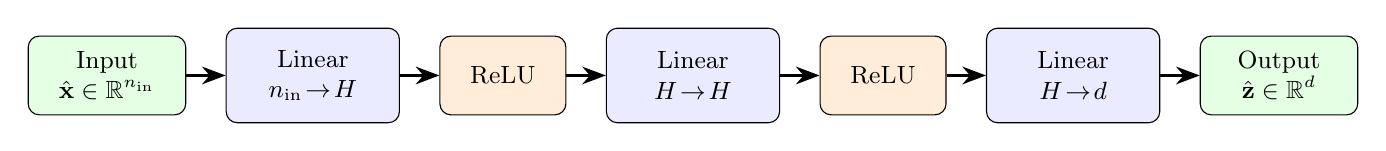
\begin{tikzpicture}[
    node distance=1.0cm and 0.5cm,
    every node/.style={font=\small},
    block/.style={rectangle, draw, rounded corners, minimum height=1.2cm,
                  minimum width=2.2cm, align=center, fill=blue!8},
    act/.style={rectangle, draw, rounded corners, minimum height=1.0cm,
                minimum width=1.6cm, align=center, fill=orange!15},
    io/.style={rectangle, draw, rounded corners, minimum height=1.0cm,
               minimum width=2.0cm, align=center, fill=green!10},
    arr/.style={-{Stealth[length=3mm]}, thick},
]

% Nodes
\node[io]    (input)  {Input\\$\hat{\bx}\in\R^{n_{\mathrm{in}}}$};
\node[block, right=of input]  (L1) {Linear\\$n_{\mathrm{in}}\!\to\!H$};
\node[act,   right=of L1]     (R1) {ReLU};
\node[block, right=of R1]     (L2) {Linear\\$H\!\to\!H$};
\node[act,   right=of L2]     (R2) {ReLU};
\node[block, right=of R2]     (L3) {Linear\\$H\!\to\!d$};
\node[io,    right=of L3]     (output) {Output\\$\hat{\bz}\in\R^{d}$};

% Arrows
\draw[arr] (input) -- (L1);
\draw[arr] (L1) -- (R1);
\draw[arr] (R1) -- (L2);
\draw[arr] (L2) -- (R2);
\draw[arr] (R2) -- (L3);
\draw[arr] (L3) -- (output);

\end{tikzpicture}
\end{center}

% ----------------------------------------------------------------------------
\subsection{Full Prediction Pipeline}
% ----------------------------------------------------------------------------

At inference, the entire CAE\,+\,MLP pipeline maps physical parameters
$(\mu, t)$ to a reconstructed spatial field
$\hat{\mathbf{u}} \in \R^{C \times H \times W}$:

\begin{center}
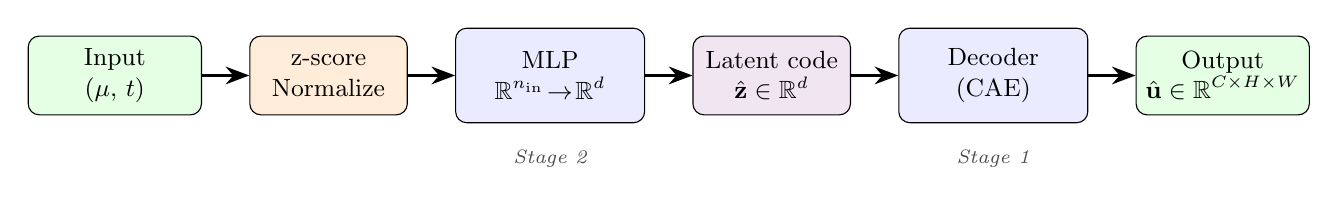
\begin{tikzpicture}[
    node distance=0.8cm and 0.6cm,
    every node/.style={font=\small},
    block/.style={rectangle, draw, rounded corners, minimum height=1.2cm,
                  minimum width=2.4cm, align=center, fill=blue!8},
    act/.style={rectangle, draw, rounded corners, minimum height=1.0cm,
                minimum width=2.0cm, align=center, fill=orange!15},
    io/.style={rectangle, draw, rounded corners, minimum height=1.0cm,
               minimum width=2.2cm, align=center, fill=green!10},
    latent/.style={rectangle, draw, rounded corners, minimum height=1.0cm,
                   minimum width=2.0cm, align=center, fill=violet!10},
    arr/.style={-{Stealth[length=3mm]}, thick},
    lbl/.style={font=\scriptsize, text=gray!70!black, above, midway},
]

% Row 1: input → normalization → MLP → latent code
\node[io]     (input)  {Input\\$(\mu,\, t)$};
\node[act,    right=of input]   (norm)   {z-score\\Normalize};
\node[block,  right=of norm]    (mlp)    {MLP\\$\R^{n_\mathrm{in}} \!\to\! \R^d$};
\node[latent, right=of mlp]     (latent) {Latent code\\$\hat{\bz} \in \R^d$};
\node[block,  right=of latent]  (dec)    {Decoder\\(CAE)};
\node[io,     right=of dec]     (output) {Output\\$\hat{\mathbf{u}} \in \R^{C \times H \times W}$};

% Arrows
\draw[arr] (input)  -- (norm);
\draw[arr] (norm)   -- (mlp);
\draw[arr] (mlp)    -- (latent);
\draw[arr] (latent) -- (dec);
\draw[arr] (dec)    -- (output);

% Stage labels
\node[font=\scriptsize\itshape, text=gray!60!black]
  at ($(mlp.south)+(0,-0.45)$) {Stage 2};
\node[font=\scriptsize\itshape, text=gray!60!black]
  at ($(dec.south)+(0,-0.45)$) {Stage 1};

\end{tikzpicture}
\end{center}

\noindent
The encoder is \emph{not} used at inference --- the MLP replaces it
entirely, producing the latent code $\hat{\bz}$ directly from the
physical parameters.  Only the frozen decoder is needed to reconstruct
the full spatial field.

% ============================================================================
\section{Training Procedure}
% ============================================================================

% ----------------------------------------------------------------------------
\subsection{Target Generation}
% ----------------------------------------------------------------------------

The MLP is \emph{not} trained on raw field data.  Instead, the frozen
Stage-1 encoder produces the training targets:
\begin{enumerate}[leftmargin=2em]
  \item Load all training snapshots $\mathbf{u}_i$ from HDF5.
  \item (Optionally) apply per-snapshot min--max normalization to $[0,1]$
    if the encoder was trained with normalization.
  \item Pass through the frozen encoder:
    $\bz_i = \mathrm{Encoder}(\mathbf{u}_i) \in \R^d$.
  \item For the KTH encoder, the latent is a spatial map
    $\bz \in \R^{z_c \times H' \times W'}$ which is flattened to a
    vector $\bz \in \R^{z_c \cdot H' \cdot W'}$.
\end{enumerate}

The MLP training data is then
$\{(\hat{\bx}_i,\; \bz_i)\}_{i=1}^{N_{\text{train}}}$.

% ----------------------------------------------------------------------------
\subsection{Loss Function}
% ----------------------------------------------------------------------------

The MLP is trained to minimize the Mean Squared Error (MSE) between
predicted and true latent codes:
\[
  \mathcal{L} = \frac{1}{N}\sum_{i=1}^{N}
  \|\hat{\bz}_i - \bz_i\|_2^2
  = \frac{1}{N}\sum_{i=1}^{N}\sum_{j=1}^{d}
  \bigl(\hat{z}_{ij} - z_{ij}\bigr)^2.
\]

% ----------------------------------------------------------------------------
\subsection{Optimizer and Learning Rate Schedule}
% ----------------------------------------------------------------------------

\begin{itemize}[leftmargin=2em]
  \item \textbf{Optimizer:} Adam with default momentum parameters
    $(\beta_1\!=\!0.9,\;\beta_2\!=\!0.999)$ and initial learning rate
    $\eta = 10^{-3}$.
  \item \textbf{Scheduler:} \texttt{ReduceLROnPlateau} ---
    if the validation loss does not decrease for 100 consecutive epochs,
    the learning rate is halved ($\eta \leftarrow 0.5\,\eta$).
  \item \textbf{Batch size:} 32.
\end{itemize}

% ----------------------------------------------------------------------------
\subsection{Early Stopping}
% ----------------------------------------------------------------------------

Training runs for up to \texttt{MAX\_EPOCHS} (5{,}000) epochs.  If the
validation loss does not improve for \texttt{PATIENCE} (500) consecutive
epochs, training stops early.  The model weights from the best validation
epoch are saved as the final model.

% ============================================================================
\section{Configurations Used in This Project}
% ============================================================================

\begin{table}[h]
\centering
\caption{MLP configurations for the two encoder types.}
\label{tab:configs}
\begin{tabular}{@{}lcc@{}}
\toprule
\textbf{Setting} & \textbf{CNN (simple\_cae)} & \textbf{KTH (resnet\_cae)} \\
\midrule
Input dim ($n_{\mathrm{in}}$) & 2 ($\mu$, $t$) & 2 ($\mu$, $t$) \\
Hidden dim ($H$)              & 64              & 64 \\
Latent dim ($d$)              & 4               & 1{,}024 \\
Total parameters              & 4{,}612         & 70{,}848 \\
Learning rate                 & $10^{-3}$       & $10^{-3}$ \\
Batch size                    & 32              & 32 \\
Max epochs                    & 5{,}000         & 5{,}000 \\
Patience                      & 500             & 500 \\
\bottomrule
\end{tabular}
\end{table}

The large difference in latent dimension (4 vs.\ 1{,}024) is because the
CNN encoder compresses to a flat 4-element vector, while the KTH
encoder uses a spatial latent map that is flattened for the MLP.

% ============================================================================
\section{What Each Component Does --- Intuition}
% ============================================================================

\paragraph{The linear layers} are learnable affine transformations.
Each neuron in a linear layer computes:
\[
  h_j = \sum_{i=1}^{n} w_{ji}\,x_i + b_j
\]
This is a weighted sum (like fitting a hyperplane).  A single linear
layer can only represent linear relationships between inputs and
outputs.

\paragraph{The ReLU activations} introduce nonlinearity by zeroing out
negative values.  This is critical: without nonlinear activations,
stacking any number of linear layers would still be equivalent to a
single linear transformation ($\bW^{(3)}\bW^{(2)}\bW^{(1)}\bx + \ldots$).
The ReLU creates piecewise-linear decision regions, enabling the network
to approximate complex nonlinear mappings.

\paragraph{Together,} the network partitions the input space into
regions (defined by which ReLU neurons are active or inactive) and
fits a different linear function in each region.  With 64 hidden
neurons per layer, the network can create up to $2^{64}$ distinct
linear regions in theory --- far more than enough to approximate
the smooth mapping $(\mu, t) \to \bz$.

\paragraph{Why no output activation?}
The target latent codes $\bz$ from the encoder are unbounded real
numbers.  Applying an activation like sigmoid or tanh at the output
would clamp predictions to a fixed range, preventing the MLP from
matching the true latent values.

\paragraph{Why is the MLP so small?}
The mapping $(\mu, t) \to \bz$ is typically smooth and low-dimensional
($\R^2 \to \R^d$).  A small MLP with $\sim$5{,}000 parameters is
sufficient.  The heavy lifting (high-dimensional spatial reconstruction)
is done by the decoder, which has millions of parameters.

% ============================================================================
\section{Numerical Worked Example}
\label{sec:example}
% ============================================================================

We trace a \emph{single} input through the entire network with concrete
numbers. To keep the arithmetic readable we use a \textbf{toy size}:
$n_{\mathrm{in}}=2$, $H=3$ (hidden), $d=2$ (latent).
The real network uses $H=64$ --- the operations are identical, just
larger matrices.

% ----------------------------------------------------------------------------
\subsection{Step 0 --- Raw physical parameters}
% ----------------------------------------------------------------------------

Suppose we want to predict the latent code for wave speed
$\mu = 1.8$ at time $t = 0.6$.  The raw input is:
\[
  \bx_{\text{raw}} = \begin{pmatrix} 1.8 \\ 0.6 \end{pmatrix}.
\]

% ----------------------------------------------------------------------------
\subsection{Step 1 --- Input normalization (z-score)}
% ----------------------------------------------------------------------------

During training, we computed the mean and standard deviation of each
input column.  Suppose:
\[
  \bar{\bx} = \begin{pmatrix} 1.5 \\ 0.5 \end{pmatrix},
  \qquad
  \boldsymbol{\sigma} = \begin{pmatrix} 0.3 \\ 0.2 \end{pmatrix}.
\]
The normalized input is computed element-wise:
\[
  \hat{x}_1 = \frac{1.8 - 1.5}{0.3} = 1.0,
  \qquad
  \hat{x}_2 = \frac{0.6 - 0.5}{0.2} = 0.5.
\]
\[
  \boxed{\hat{\bx} = \begin{pmatrix} 1.0 \\ 0.5 \end{pmatrix}}
\]
This is what actually enters the network.  Every input feature now has
a similar scale, regardless of its physical units.

% ----------------------------------------------------------------------------
\subsection{Step 2 --- Layer 1: Linear ($2 \to 3$)}
% ----------------------------------------------------------------------------

The first linear layer has a weight matrix
$\bW^{(1)} \in \R^{3 \times 2}$ and bias $\bb^{(1)} \in \R^3$.
Suppose the trained weights are:
\[
  \bW^{(1)} =
  \begin{pmatrix}
     0.6 & -0.4 \\
    -0.3 &  0.8 \\
     0.5 &  0.5
  \end{pmatrix},
  \qquad
  \bb^{(1)} =
  \begin{pmatrix} 0.1 \\ -0.2 \\ 0.0 \end{pmatrix}.
\]
Each row of $\bW^{(1)}$ defines one hidden neuron.  The computation is:
\begin{align}
  h^{(1)}_1 &= w_{11}\,\hat{x}_1 + w_{12}\,\hat{x}_2 + b_1
             = (0.6)(1.0) + (-0.4)(0.5) + 0.1
             = 0.6 - 0.2 + 0.1
             = \mathbf{0.5}, \notag \\[4pt]
  h^{(1)}_2 &= w_{21}\,\hat{x}_1 + w_{22}\,\hat{x}_2 + b_2
             = (-0.3)(1.0) + (0.8)(0.5) + (-0.2)
             = -0.3 + 0.4 - 0.2
             = \mathbf{-0.1}, \notag \\[4pt]
  h^{(1)}_3 &= w_{31}\,\hat{x}_1 + w_{32}\,\hat{x}_2 + b_3
             = (0.5)(1.0) + (0.5)(0.5) + 0.0
             = 0.5 + 0.25
             = \mathbf{0.75}. \notag
\end{align}
In matrix form:
\[
  \bh^{(1)} = \bW^{(1)}\hat{\bx} + \bb^{(1)}
  = \begin{pmatrix} 0.5 \\ -0.1 \\ 0.75 \end{pmatrix}.
\]

% ----------------------------------------------------------------------------
\subsection{Step 3 --- Activation 1: ReLU}
% ----------------------------------------------------------------------------

ReLU is applied element-wise: $\max(0,\; h_j)$.
\begin{align}
  \text{ReLU}(0.5)  &= \max(0,\; 0.5)  = \mathbf{0.5}
    \qquad\text{(positive $\to$ passes through)}, \notag \\[3pt]
  \text{ReLU}(-0.1) &= \max(0,\;\! -0.1) = \mathbf{0.0}
    \qquad\text{(negative $\to$ killed to zero)}, \notag \\[3pt]
  \text{ReLU}(0.75) &= \max(0,\; 0.75) = \mathbf{0.75}
    \qquad\text{(positive $\to$ passes through)}. \notag
\end{align}
\[
  \boxed{\bh^{(1)}_{\text{act}} = \begin{pmatrix} 0.5 \\ 0.0 \\ 0.75 \end{pmatrix}}
\]

\textbf{Key observation:} Neuron~2 is ``dead'' for this input ---
its output is zero and it contributes nothing to downstream
computations.  Different inputs will activate different subsets of
neurons, creating the piecewise-linear behavior discussed earlier.

% ----------------------------------------------------------------------------
\subsection{Step 4 --- Layer 2: Linear ($3 \to 3$)}
% ----------------------------------------------------------------------------

The second linear layer has $\bW^{(2)} \in \R^{3 \times 3}$ and
$\bb^{(2)} \in \R^3$.  Suppose:
\[
  \bW^{(2)} =
  \begin{pmatrix}
     0.4 &  0.2 & -0.6 \\
    -0.5 &  0.7 &  0.3 \\
     0.1 & -0.3 &  0.9
  \end{pmatrix},
  \qquad
  \bb^{(2)} =
  \begin{pmatrix} 0.05 \\ 0.10 \\ -0.05 \end{pmatrix}.
\]
Since $h^{(1)}_{\text{act},2} = 0$, the second column of $\bW^{(2)}$
is multiplied by zero and has no effect:
\begin{align}
  h^{(2)}_1 &= (0.4)(0.5) + (0.2)(0.0) + (-0.6)(0.75) + 0.05
             = 0.2 + 0 - 0.45 + 0.05
             = \mathbf{-0.2}, \notag \\[4pt]
  h^{(2)}_2 &= (-0.5)(0.5) + (0.7)(0.0) + (0.3)(0.75) + 0.10
             = -0.25 + 0 + 0.225 + 0.10
             = \mathbf{0.075}, \notag \\[4pt]
  h^{(2)}_3 &= (0.1)(0.5) + (-0.3)(0.0) + (0.9)(0.75) + (-0.05)
             = 0.05 + 0 + 0.675 - 0.05
             = \mathbf{0.675}. \notag
\end{align}
\[
  \bh^{(2)} = \begin{pmatrix} -0.2 \\ 0.075 \\ 0.675 \end{pmatrix}.
\]

% ----------------------------------------------------------------------------
\subsection{Step 5 --- Activation 2: ReLU}
% ----------------------------------------------------------------------------

\begin{align}
  \text{ReLU}(-0.2)  &= \mathbf{0.0}
    \qquad\text{(killed)}, \notag \\[3pt]
  \text{ReLU}(0.075) &= \mathbf{0.075}
    \qquad\text{(passes)}, \notag \\[3pt]
  \text{ReLU}(0.675) &= \mathbf{0.675}
    \qquad\text{(passes)}. \notag
\end{align}
\[
  \boxed{\bh^{(2)}_{\text{act}} = \begin{pmatrix} 0.0 \\ 0.075 \\ 0.675 \end{pmatrix}}
\]

Now neuron~1 is dead (different from Layer~1 where neuron~2 was dead).
This shows how the ``active region'' changes from layer to layer.

% ----------------------------------------------------------------------------
\subsection{Step 6 --- Layer 3: Output Linear ($3 \to 2$)}
% ----------------------------------------------------------------------------

The final layer maps to the latent dimension $d=2$.
$\bW^{(3)} \in \R^{2 \times 3}$, $\bb^{(3)} \in \R^2$.  Suppose:
\[
  \bW^{(3)} =
  \begin{pmatrix}
    0.3 & -0.8 &  1.2 \\
    0.7 &  0.4 & -0.5
  \end{pmatrix},
  \qquad
  \bb^{(3)} =
  \begin{pmatrix} 0.02 \\ -0.01 \end{pmatrix}.
\]
\begin{align}
  \hat{z}_1 &= (0.3)(0.0) + (-0.8)(0.075) + (1.2)(0.675) + 0.02
             = 0 - 0.06 + 0.81 + 0.02
             = \mathbf{0.77}, \notag \\[4pt]
  \hat{z}_2 &= (0.7)(0.0) + (0.4)(0.075) + (-0.5)(0.675) + (-0.01)
             = 0 + 0.03 - 0.3375 - 0.01
             = \mathbf{-0.3175}. \notag
\end{align}
\[
  \boxed{\hat{\bz} = \begin{pmatrix} 0.77 \\ -0.3175 \end{pmatrix}}
  \quad\longleftarrow\;\text{predicted latent code (no activation!)}
\]

Note that $\hat{z}_2$ is \emph{negative} --- this is perfectly fine
because there is no output activation to clamp the values.

% ----------------------------------------------------------------------------
\subsection{Complete Forward Pass Summary}
% ----------------------------------------------------------------------------

\[
\underbrace{\begin{pmatrix} 1.8 \\ 0.6 \end{pmatrix}}_{\text{raw } (\mu,t)}
\xrightarrow{\text{z-score}}
\underbrace{\begin{pmatrix} 1.0 \\ 0.5 \end{pmatrix}}_{\hat{\bx}}
\xrightarrow{\bW^{(1)}\hat{\bx}+\bb^{(1)}}
\underbrace{\begin{pmatrix} 0.5 \\ \!\!-0.1 \\ 0.75 \end{pmatrix}}_{\bh^{(1)}}
\xrightarrow{\text{ReLU}}
\underbrace{\begin{pmatrix} 0.5 \\ 0.0 \\ 0.75 \end{pmatrix}}_{\bh^{(1)}_\text{act}}
\]
\[
\xrightarrow{\bW^{(2)}\bh+\bb^{(2)}}
\underbrace{\begin{pmatrix} \!\!-0.2 \\ 0.075 \\ 0.675 \end{pmatrix}}_{\bh^{(2)}}
\xrightarrow{\text{ReLU}}
\underbrace{\begin{pmatrix} 0.0 \\ 0.075 \\ 0.675 \end{pmatrix}}_{\bh^{(2)}_\text{act}}
\xrightarrow{\bW^{(3)}\bh+\bb^{(3)}}
\boxed{\hat{\bz} = \begin{pmatrix} 0.77 \\ -0.3175 \end{pmatrix}}
\]

% ----------------------------------------------------------------------------
\subsection{What Happens Next}
% ----------------------------------------------------------------------------

This predicted latent code $\hat{\bz}$ is passed to the Stage-1
\textbf{Decoder} to reconstruct the full spatial field:
\[
  \hat{\bz} = \begin{pmatrix} 0.77 \\ -0.3175 \end{pmatrix}
  \;\xrightarrow{\;\text{Decoder}\;}\;
  \hat{\mathbf{u}} \in \R^{1 \times 256 \times 256}
\]
The decoder (a large convolutional network with millions of parameters)
maps this tiny 2-element vector back to the $256\times256$ field ---
that is the power of the learned latent representation.

% ----------------------------------------------------------------------------
\subsection{Scaling to the Real Network}
% ----------------------------------------------------------------------------

In the actual network ($H=64$, $d=4$), the operations are identical:
\begin{itemize}[leftmargin=2em]
  \item Layer~1 multiplies a $(64\times2)$ matrix by the 2-element input
    $\to$ 64 pre-activations, then ReLU zeros out some of the 64.
  \item Layer~2 multiplies a $(64\times64)$ matrix by the 64-element vector
    $\to$ 64 pre-activations, then ReLU zeros out some.
  \item Layer~3 multiplies a $(4\times64)$ matrix by the 64-element vector
    $\to$ the final 4 latent code values.
\end{itemize}
The only difference is the size of the matrices --- the algebra is the
same as shown above, just with larger vectors.

\end{document}
